\documentclass[crop,tikz]{standalone}
\usepackage{physics}
\usepackage{amsmath, bm, bbm}
\usetikzlibrary{positioning}
\usetikzlibrary{decorations.pathreplacing,calligraphy}

\usepackage{pgfplots}
\usetikzlibrary{intersections, pgfplots.fillbetween}

\begin{document}
\begin{tikzpicture}[
node/.style={shape=rectangle, rounded corners=.1cm, draw=black, line width=1, fill=black!10},
edge/.style={-latex, thick},
every text node part/.style={align=center}
]


        \draw[name path=A] (-8, 3) rectangle (9, -5.2);
        \draw[name path=B] (-8.2, 3.2) rectangle (9.2, -5.4);
        \tikzfillbetween[of=A and B] {black, opacity=0.5};
        \node[shape=rectangle, rounded corners, fill=white, draw=black, minimum width=3.2cm, minimum height=0.7cm] (title) at (0, 2.7) {RIM baseline $\varphi_\mathcal{D}^{\star}$}; 

        \node at (-6, 1.4) {Background source \\ $\mathbf{s}$};
        \node at (-3, 1.4) {Foreground lens \\ $\boldsymbol{\kappa}$};
        \node (source) at (-6, 0) {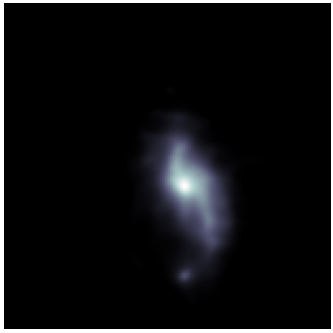
\includegraphics[height=2cm]{source_highlight}};
        \node (kappa) at (-3, 0) {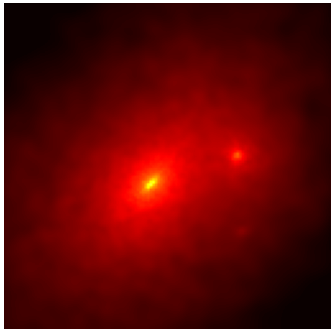
\includegraphics[height=2cm]{kappa_highlight}};
        \draw (-7.1, 1) .. controls (-7.3, 0.5) and (-7.3, -0.5) .. (-7.1, -1);
        \draw (-1.8, 1) .. controls (-1.6, 0.5) and (-1.6, -0.5) .. (-1.8, -1);
        \node at (-4.5, -1) {\huge ,};
        \node at (-7.6, 0) {\huge $F$};
        \node at (1, 0) {\huge $=$};
        \node at (-1, 0) {\huge $+$};
        \node at (0, 0) {\huge $\boldsymbol{\eta}$};
        \node at (3, 1.4) {Simulated observation \\ $\mathbf{y}$};
        \node (obs) at (3, 0) {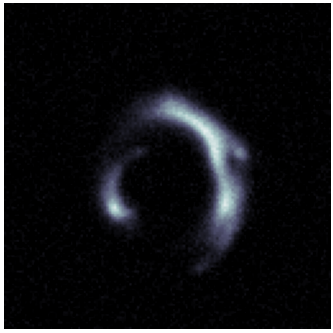
\includegraphics[height=2cm]{observation_highlight}};

        \draw[-latex, thick] (obs.south) .. controls +(0, -1) and +(0, 1) .. (-4.5, -2.2) node[midway, below] {$G_{\varphi_{\mathcal{D}}^{\star}}$}; 

        \node (s_hat) at (-6, -2.8) {$\mathbf{\hat{s}}^{(T)}$};
        \node (source_pred) at (-6, -4) {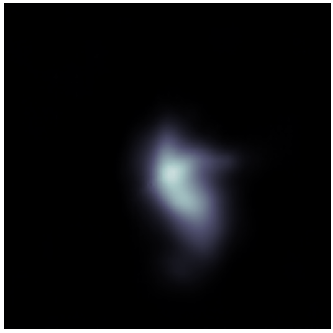
\includegraphics[height=2cm]{source_pred_highlight}};
        \node (k_hat) at (-3, -2.8) {$\boldsymbol{\hat{\kappa}}^{(T)}$};
        \node (kappa_pred) at ( -3, -4) {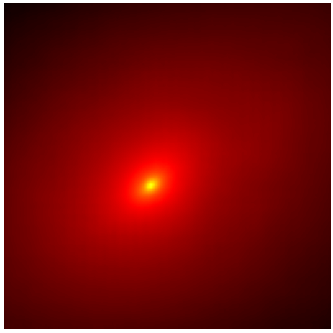
\includegraphics[height=2cm]{kappa_pred_highlight}};
        \draw (-7.1, -3) .. controls (-7.3, -3.5) and (-7.3, -4.5) .. (-7.1, -5);
        \draw (-1.8, -3) .. controls (-1.6, -3.5) and (-1.6, -4.5) .. (-1.8, -5);
        \node at (-4.5, -5) {\huge ,};
        \node at (-7.6, -4) {\huge $F$};
        \node at (1, -4) {\huge $=$};
        \node at (3, -2.8) {$\mathbf{\hat{y}}^{(T)}$};
        \node (obs_pred) at (3, -4) {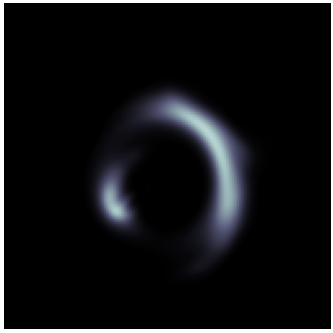
\includegraphics[height=2cm]{observation_pred_highlight}};

        \node (res) at (7.5, -2) {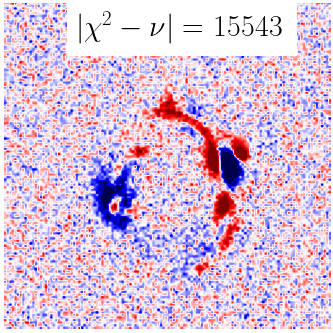
\includegraphics[height=2cm]{residual_highlight}};
        \node at (7.5, -0.5) {Normalized \\ residuals};
        \draw[-latex, thick, in=180, out=0] (obs.east) to (res.west);
        \draw[-latex, thick, in=180, out=0] (obs_pred.east) to (res.west);


        %\node (samples1) at (-5, -9) {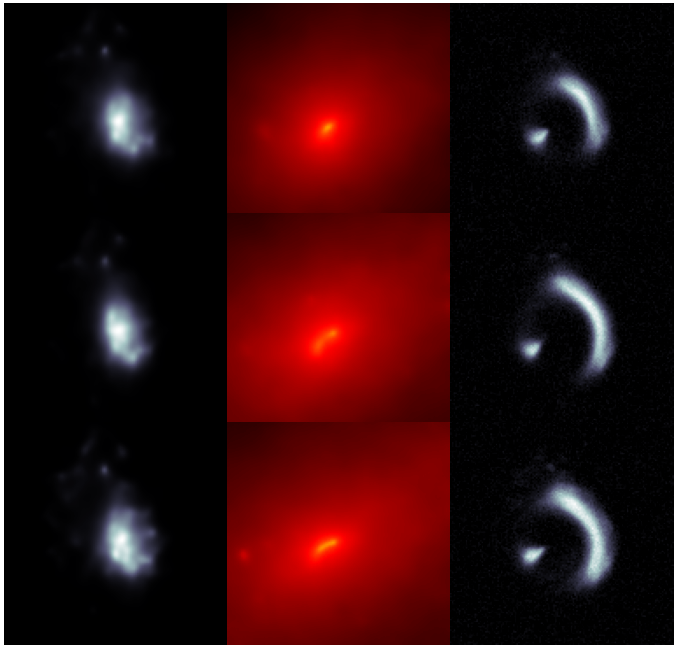
\includegraphics[height=3cm]{highlight_vae_samples1}};
        \filldraw[thick, fill=black!40] (-7, -6.7) -- (-5, -6.7) -- (-5.5, -7.9) -- (-6.5, -7.9) -- cycle;
        \filldraw[thick, fill=red!40] (-4, -6.7) -- (-2, -6.7) -- (-2.5, -7.9) -- (-3.5, -7.9) -- cycle;
        \node at (-4.5, -6.9) {VAE};
        \node at (-4.5, -7.4) {Encoder};
        \node (samples2) at (-4.5, -13.4) {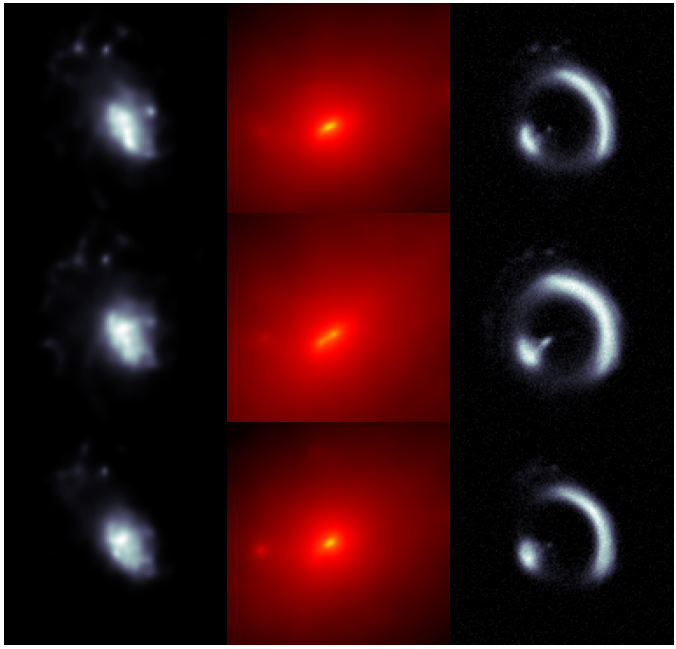
\includegraphics[height=4cm]{highlight_vae_samples2}};

        \filldraw[thick, fill=black!20] (-6, -8.6) circle (14pt);
        \node[thick, fill=black, draw=black, minimum size=2pt, circle] (zs) at (-6.2, -8.6) {};

        \node at (-4.5, -8.4) {Latent};
        \node at (-4.5, -9) {Space};

        \filldraw[thick, fill=red!20] (-3, -8.6) circle (14pt);
        \node[thick, fill=red, draw=black, circle, minimum size=1pt] (zk) at (-2.8, -8.7) {};

        \filldraw[thick, fill=black!40] (-7, -10.7) -- (-5, -10.7) -- (-5.5, -9.4) -- (-6.5, -9.4) -- cycle;
        \filldraw[thick, fill=red!40] (-4, -10.7) -- (-2, -10.7) -- (-2.5, -9.4) -- (-3.5, -9.4) -- cycle;

        \node at (-4.5, -9.9) {Decoder};

        \draw[-latex, red, thick] (kappa_pred) -- (-3, -6.7);
        \draw[-latex, thick] (source_pred) -- (-6, -6.7);

        \draw[-latex, thick] (-6, -7.9) to (zs);
        \draw[-latex, red, thick] (-3, -7.9) to (zk);

        \draw[-latex, thick, red] (zk) to (-3, -9.4);
        \draw[-latex, thick] (zs) to (-6, -9.4);


        \node (source_pred_reoptim) at (7.5, -8.4) {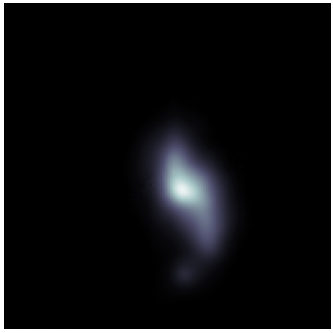
\includegraphics[height=2cm]{source_pred_reoptim_highlight}};
        \node (kappa_pred_reoptim) at (7.5, -10.4) {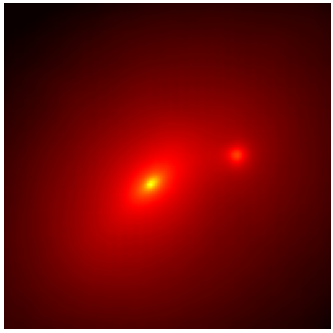
\includegraphics[height=2cm]{kappa_pred_reoptim_highlight}};
        \node (obs_pred_roptim) at (7.5, -12.4) {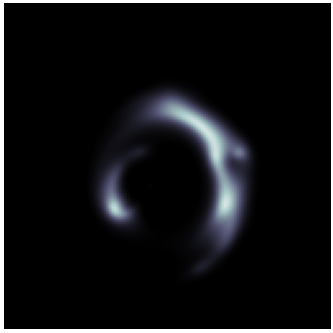
\includegraphics[height=2cm]{observation_pred_reoptim_highlight}};
        \node (res_reoptim) at (7.5, -14.4) {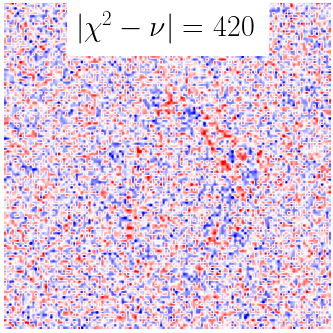
\includegraphics[height=2cm]{residual_reoptim_highlight}};

        \draw[-latex, thick, red] (-3, -10.7) .. controls +(0, -0.5) and +(0, 0.5) .. (-4.5, -11.4);
        \draw[-latex, thick] (-6, -10.7) .. controls +(0, -0.5) and +(0, 0.5) .. (-6, -11.4);
        
        \node[rounded corners, minimum size=2cm] (N) at (1.2, -13.4) 
                {Generate $N$ similar lensing systems \\[4pt] 
                        from $\tilde{p}(\mathcal{D}^{\mathrm{train}} \mid \mathcal{T})$\\[4pt]
                        to estimate $[\mathcal{I}(\varphi_{\mathcal{D}}^{\star})]_{jj}$
        };
        %\node at (-4.5, -16) {};

        \node at (2, -9) {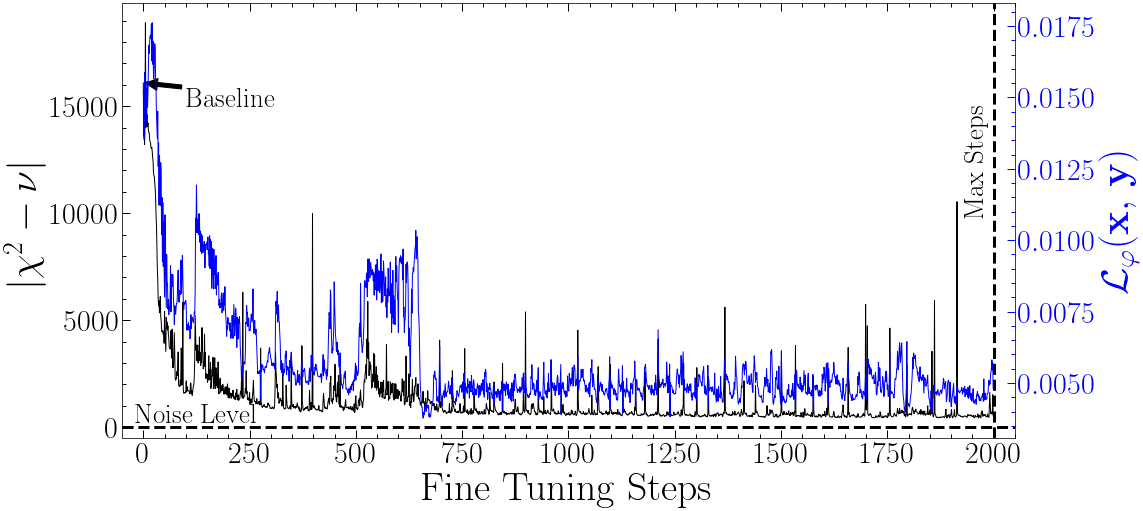
\includegraphics[width=8cm]{highlight_loss_curve}};

        \draw[decorate, decoration={brace, amplitude=10pt, aspect=0.5, raise=-5pt}] (-2.1, -11.4) -- (-2.1, -15.4);

        %\node[rounded corners, fill=black!20, minimum size=1cm] (fisher) at (0, -11.5) 
                %{Compute $[\mathcal{I}(\varphi_{\mathcal{D}}^{\star})]_{jj}$};
        %\draw[-latex, thick] (N) to (fisher);
        %\draw[-latex, thick] (fisher.north) -- ++(0, 0.6);
        %\draw[-latex, thick] (4.6, -9.8) .. controls +(1, 0) and +(-1.5, 0) .. (6, -11);

        \node[rounded corners, minimum size=1cm] at (2, -7) {Optimize Likelihood + EWC};
        \node at (7.5, -6.8) {Fine-tuned \\ prediction};

        \draw[name path=C] (-8, -5.6) rectangle (9, -15.7);
        \draw[name path=D] (-8.2, -5.4) rectangle (9.2, -15.9);
        \tikzfillbetween[of=C and D] {red, opacity=0.5};
        \node[shape=rectangle, rounded corners, draw=black, fill=white, minimum width=3.2cm, minimum height=0.7cm] (likelihood title) at (0, -5.9) {Fine-tuning $\hat{\varphi}_{\mathrm{MAP}}$};





\end{tikzpicture}
\end{document}
